\documentclass[tikz]{standalone}
\usepackage{tikz-3dplot}

\begin{document}

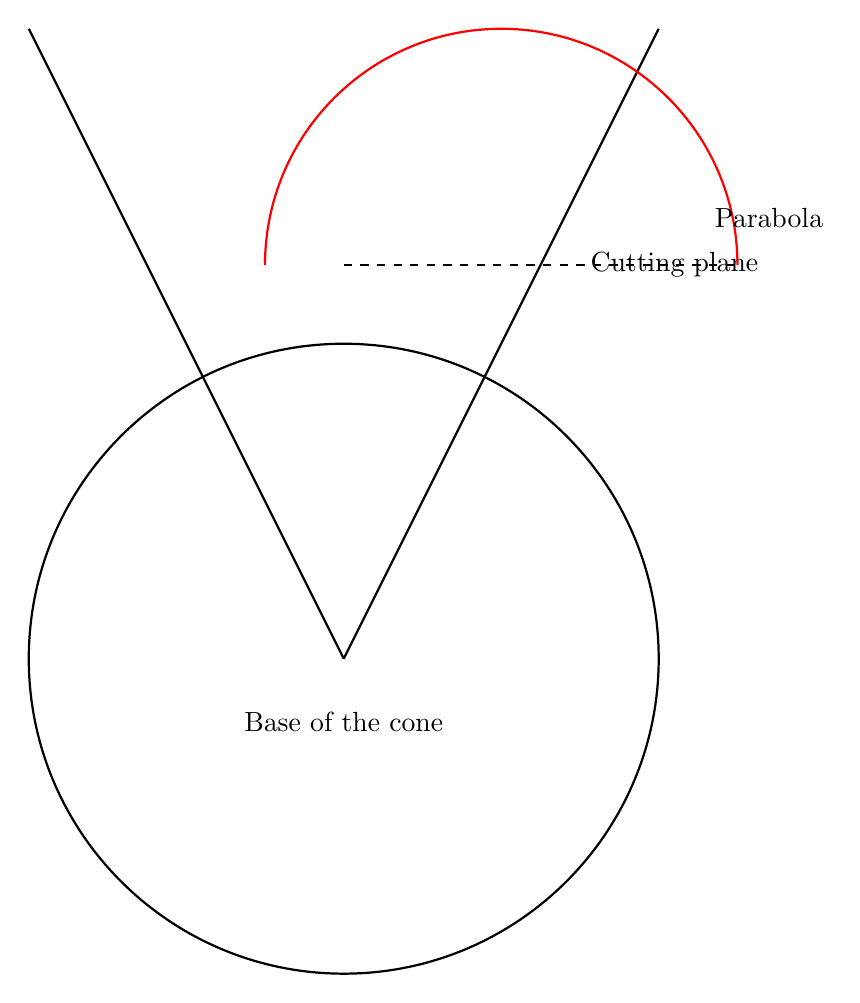
\begin{tikzpicture}[scale=2]

% Coordinates for the cone
\def\coneheight{4} % height of the cone
\def\coneradius{2} % radius of the cone base
\def\planeheight{2.5} % height at which the plane cuts the cone

% Draw the cone's base (ellipse projected in 3D)
\draw[thick] (0,0) circle (\coneradius);

% Draw the cone sides by drawing lines from the apex to the edge of the base
\draw[thick] (0,0) -- (\coneradius,\coneheight); % Right slant
\draw[thick] (0,0) -- (-\coneradius,\coneheight); % Left slant

% Draw the cutting plane: a line intersecting the cone
\draw[thick, dashed] (0, \planeheight) -- (\planeheight,\planeheight); % Parabola cut section

% Red parabola section of the cone
\draw[thick, red] (\planeheight,\planeheight) arc[start angle=0,end angle=180,radius=1.5];

% Labels
\node at (0,-0.4) {Base of the cone};
\node at (\planeheight-0.4, 2.5) {Cutting plane};
\node at (\planeheight+0.2, 2.8) {Parabola};

\end{tikzpicture}

\end{document}

